\documentclass[../main.tex]{subfiles}

\begin{document}

\section{Altimetría}
Con los datos de la altimetría se comenzó proponiendo una traza tentativa (que luego será verificada) en función a los elementos existentes que demandaban puntos obligados altimétricamente. De la misma, se extrajeron las pendientes y vértices de las curvas verticales

\subsection{Estudios Generales}

\subsubsection{Diferencia de pendientes}
Se calcula la diferencia entre las pendientes $i_1$ e $i_2$, lo que define la diferencia de pendientes geométrica:

\begin{equation}
    i_0 = i_2 - i_1
\end{equation}


\subsubsection{Parámetro mínimo }

Extraemos el parámetro mínimo del índice General de Tablas (cita viguria). Luego obtenemos la longitud de la curva como:

\begin{equation}
    L = \frac{P_{min} * i_0}{100}
\end{equation}


\subsubsection{Longitud Mínima}

La longitud mínima de la curva vertical se determinó como la mayor de los siguientes valores.\cite{cornero_altimetria}

\begin{itemize}
    \item \textbf{Según confort de la circulación:} $L=v_d^2*i_o/390$ 
    \item \textbf{Según apariencia estética:} según lo indica la tabla 3.2 $L=06*V_d$ 
    \item \textbf{Según apariencia estética:} según lo indica la tabla 3.2 $L=0,6 V_d$ 
    \item \textbf{Según visibilidad de frenado}: se obtienen dos procedimientos para determinar esta longitud. El primero, interpolando los valores de pendiente y longitud según las tablas del Anexo I, y el segundo según la expresión $L=2*D-(426/i_o)$, siendo $D$ la distancia de frenado obtenida de la tabla 3.1. 
    \item \textbf{Según la visibilidad de sobrepaso:} este ítem no fue tenido en cuenta en la determinación de la longitud mínima puesto que se requieren longitudes que escapan de la tabla y gráfico 3.1. Debido a esto se optó por proyectar la señalización correspondiente. 
\end{itemize}


Elegida la longitud mínima se vuelve a calcular el Parámetro Mínimo mediante:

\begin{equation}
P_{min}= \frac{L_{min}*100}{i_0}
\end{equation}

Después se busca el inmediato superior en las tablas de Viguria. Finalmente se adopta la longitud de la curva para el Parámetro Mínimo calculado. 


\subsection{Estudios de Puntos Singulares}

Finalizado el estudio general se analizan dos puntos importantes (inicio y fin de la curva vertical), definidos como Punto A y Punto B y la excentricidad en el vértice.

\textbf{Punto A:}
\begin{align}
X_a &= X_0 - L/2 \\
Y_a &= Y_0 - (i_1 * L/2)
\end{align}

\textbf{Punto B}
\begin{align}
X_a &= X_0 + L/2 \\
Y_a &= Y_0 - (i_2 * L/2)
\end{align}

\textbf{Excentricidad }
\begin{equation}
e = \frac{i_0 * L}{800}
\end{equation}

\subsection{Estudio de Cotas}
Para el estudio de cotas se utilizaron dos procedimientos, el primero mediante curvas ya tabuladas, en el cual, con las pendientes se determina un plano de comparación (P.C), luego se calcula la progresiva de la tabla como la progresiva origen más la distancia hasta la progresiva actual, finalmente se busca ese valor en la correspondiente tabla de Viguria y se lo suma al plano de comparación. Por otro lado, el segundo método consiste en sumarle (curva cóncava) o restarle (curva convexa) el valor de la excentricidad a la cota que posee cada progresiva según su pendiente. Primero, partimos de los siguientes datos:

\begin{figure}
    \centering
    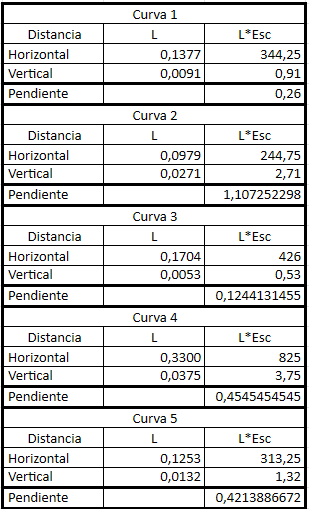
\includegraphics{images/google_sheets/Screenshot_8.png}
    \caption{Pendientes geométricas}
    \label{fig:pendientes}
\end{figure}
\subsubsection{Curva 1}
Los valores obtenidos son:

\begin{align*}
    L_{min} = 110 \text{m} \\
    P_{min} = 13095
\end{align*}

Con lo anterior, adoptamos los siguientes valores:

\begin{align*}
    P = 14285,71  \\
    L = 120
\end{align*}

El estudio de los puntos singulares nos dan los siguientes valores:

\textbf{Punto A}
\begin{align*}
    X_a = 432204 \text{m} \\
    Y_a = 57,95 \text{m}
\end{align*}

\textbf{Punto B}
\begin{align*}
    X_a = 432324 \text{m} \\
    Y_a = 57,13 \text{m}
\end{align*}

Y la excentricidad nos dió:

\begin{equation*}
    e = 0,13 \text{m}
\end{equation*}

Luego, podemos resolver lo siguiente:

\begin{figure}[h]
    \centering
    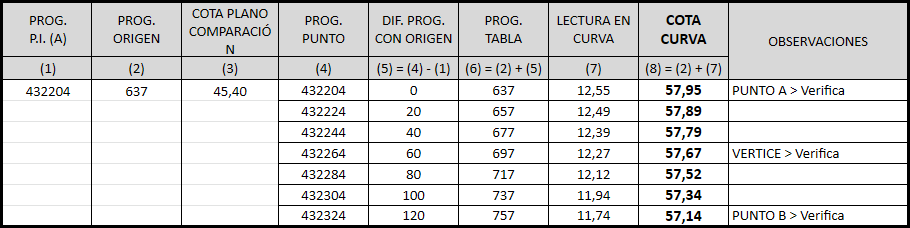
\includegraphics[width=\textwidth]{images/google_sheets/Screenshot_10.png}
    \caption{Cálculo curva Nº1}
    \label{fig:curva1-1}
\end{figure}

\begin{figure}[h]
    \centering
    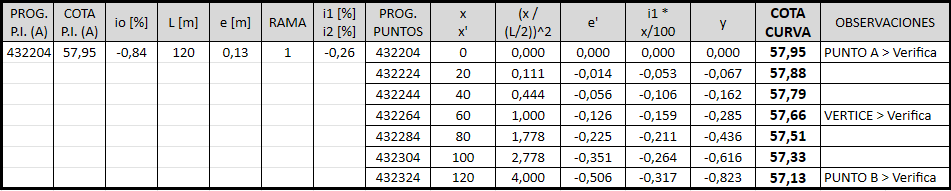
\includegraphics[width=\textwidth]{images/google_sheets/Screenshot_11.png}
    \caption{Cálculo curva Nº1}
    \label{fig:curva1-2}
\end{figure}

\subsubsection{Curva 2}
Los valores obtenidos son:

\begin{align*}
    L_{min} = 116 \text{m} \\
    P_{min} = 11803
\end{align*}

Con lo anterior, adoptamos los siguientes valores:

\begin{align*}
    P = 14285,71 \\
    L = 140
\end{align*}

El estudio de los puntos singulares nos dan los siguientes valores:

\textbf{Punto A}
\begin{align*}
    X_a = 432439 \text{m} \\
    Y_a = 55,86 \text{m}
\end{align*}

\textbf{Punto B}
\begin{align*}
    X_a = 432580 \text{m} \\
    Y_a = 54,99 \text{m}
\end{align*}

Y la excentricidad nos dió:

\begin{equation*}
    e = -0,17 \text{m}
\end{equation*}

Luego, podemos resolver lo siguiente:

\begin{figure}[h]
    \centering
    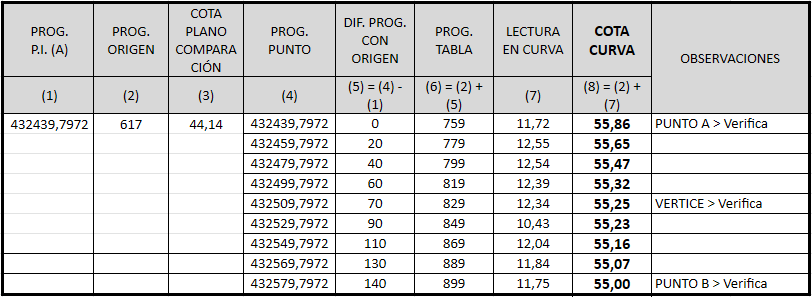
\includegraphics[width=\textwidth]{images/google_sheets/Screenshot_12.png}
    \caption{Cálculo curva Nº2}
    \label{fig:curva2-1}
\end{figure}

\begin{figure}[h]
    \centering
    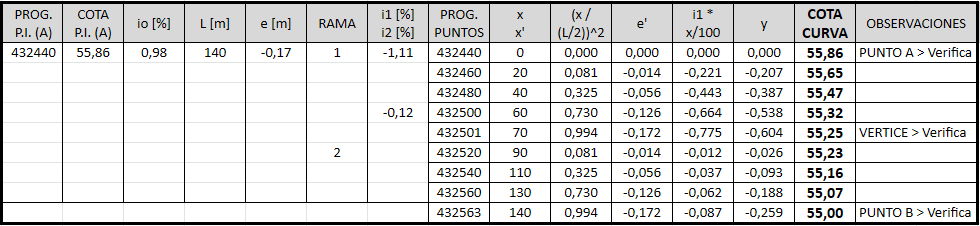
\includegraphics[width=\textwidth]{images/google_sheets/Screenshot_13.png}
    \caption{Cálculo curva Nº2}
    \label{fig:curva2-2}
\end{figure}

\subsubsection{Curva 3}
Los valores obtenidos son:

\begin{align*}
    L_{min} = 103 \text{m} \\
    P_{min} = 17791
\end{align*}

Con lo anterior, adoptamos los siguientes valores:

\begin{align*}
    P = 20000 \\
    L = 120
\end{align*}

El estudio de los puntos singulares nos dan los siguientes valores:

\textbf{Punto A}
\begin{align*}
    X_a = 432876 \text{m} \\
    Y_a = 54,62 \text{m}
\end{align*}

\textbf{Punto B}
\begin{align*}
    X_a = 432996 \text{m} \\
    Y_a = 54,82 \text{m}
\end{align*}

Y la excentricidad nos dió:

\begin{equation*}
    e = 0,09 \text{m}
\end{equation*}

Luego, podemos resolver lo siguiente:

\begin{figure}[h]
    \centering
    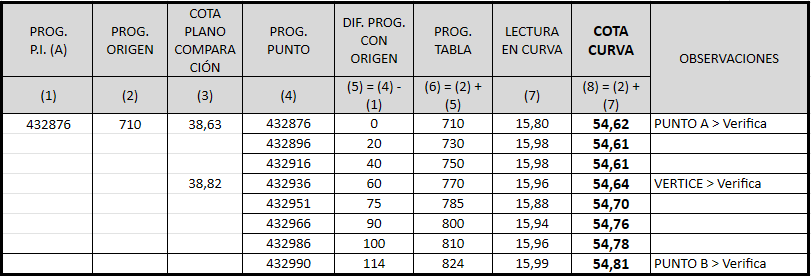
\includegraphics[width=\textwidth]{images/google_sheets/Screenshot_14.png}
    \caption{Cálculo curva Nº3}
    \label{fig:curva3-1}
\end{figure}

\begin{figure}[h]
    \centering
    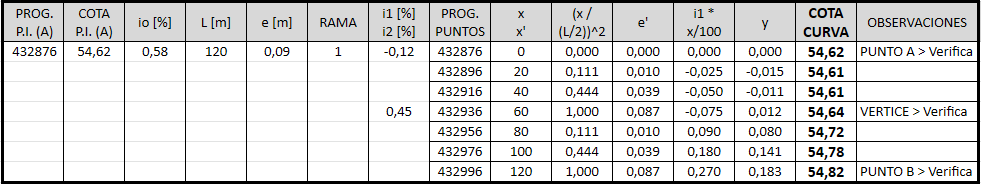
\includegraphics[width=\textwidth]{images/google_sheets/Screenshot_15.png}
    \caption{Cálculo curva Nº3}
    \label{fig:curva3-2}
\end{figure}

\subsubsection{Curva 4}
Los valores obtenidos son:

\begin{align*}
    L_{min} = 120 \text{m} \\
    P_{min} = 13700
\end{align*}

Con lo anterior, adoptamos los siguientes valores:

\begin{align*}
    L = 125 \\
    P = 14285,71 
\end{align*}

El estudio de los puntos singulares nos dan los siguientes valores:

\textbf{Punto A}
\begin{align*}
    X_a = 433698 \text{m} \\
    Y_a = 58,04 \text{m}
\end{align*}

\textbf{Punto B}
\begin{align*}
    X_a = 433823 \text{m} \\
    Y_a = 58,04 \text{m}
\end{align*}

Y la excentricidad nos dio:

\begin{equation*}
    e = -0,14 \text{m}
\end{equation*}

Luego, podemos resolver lo siguiente

\begin{figure}[h]
    \centering
    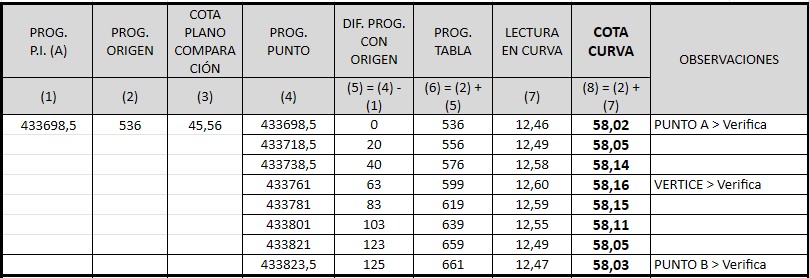
\includegraphics[width=\textwidth]{images/google_sheets/Screenshot_16.png}
    \caption{Cálculo curva Nº4}
    \label{fig:curva4-1}
\end{figure}

\begin{figure}[h]
    \centering
    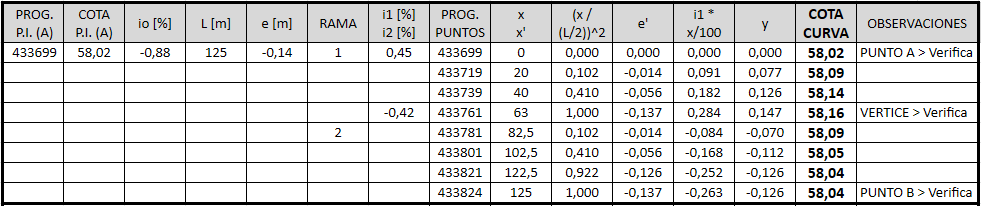
\includegraphics[width=\textwidth]{images/google_sheets/Screenshot_17.png}
    \caption{Cálculo curva Nº4}
    \label{fig:curva4-2}
\end{figure}






\end{document}